\documentclass[12pt]{report}
\renewcommand{\baselinestretch}{1.2}
\usepackage[utf8]{inputenc}
\usepackage{amsmath,mathtools}
\usepackage{tcolorbox}
\newcommand{\mbf}[1]{\mathbf{#1}}
\newcommand{\tbf}[1]{\textbf{#1}}
\newcommand{\dsum}[3]{$\sum^{#1}_{#2}{#3}$}
\newcommand{\dint}[3]{\int^{#1}_{#2}{#3}}
\newcommand{\tit}[1]{\textit{#1}}
\newcommand{\fn}[1]{\footnote{#1}}
\newcommand{\de}[2]{\frac{d{#1}}{d{#2}}}
\newcommand{\ch}[2]{\Gamma^{#1}_{#2}}
\newcommand{\chris}{\ch{\mu}{\alpha \beta}=\frac{1}{2}g^{\mu \lambda}(\p_{\alpha} g_{\beta \lambda}+\p_\beta g_{\alpha \lambda} - \p_\lambda g_{\alpha \beta})}
\newcommand{\p}{\partial}
\newcommand{\pe}[2]{\frac{\partial{#1}}{\partial{#2}}}
\newcommand{\n}{\nonumber}
\newcommand{\cbox}{tcolorbox}
\newcommand{\cc}[1]{\left({#1}\right)}
\newcommand{\rr}[1]{\left[{#1}\right]}
\newcommand{\vd}[1]{\dot{\vec{#1}}}
\newcommand{\tx}[1]{\text{#1}}
\begin{document}
\title{Cluster Mergers}
\author{Divesh Jain}
\maketitle
\tableofcontents

\chapter{Introduction}
The idea of this document is to basically cover all theoretical aspects of areas and bootstrapping related to Ruta's project. 
\begin{itemize}
\item Understanding theory behind radiation
\item cover synchrotron and review papers eventually
\item How shocks lead to Cosmic Rays(finding a connection between radio and X-ray) - \textbf{Read VanWeeren Review}
\item The type of mechanism involved in particle acceleration(Fermi I and Fermi II Order acceleration ) - \textbf{Read Brunetti Review}
\end{itemize}
Over many areas, one area I am thoroughly interested is in particle acceleration mechanism.
\chapter{Basics behind Radiation}
\section{Principles of Special Relativity}
To describe a physical process we require both spatial and temporal co-ordinates of the events, which can be put to a single entity of four numbers $x^i=(t,\mbf{x})$. For the purpose of this article and following sections to come Latin indices \tit{a,b,c..,i,j,k} run over 0 , 1, 2 and 3; where 1, 2, 3 denote space dimensions.The Greek indices would be used to represent just the spatial dimensions.\\

In the following discussion we pay special attention to a subset of coordinate systems, called \textbf{inertial coordinate systems.} \\
\textbf{How do we create this inertial coordinate system?}\\
These coordinates systems, are defined by the property that a material particle, far removed from all external influences, will move with uniform velocities in such systems. verify this criterion. \textbf{But, there is no fundamental reason why any one class of coordinate systems should be preferred over others except for mathematical convenience.}Just to make our lives simpler, we still postulate that such a set of coordinates exists where any frame moves with uniform velocity with respect to an inertial frame.\\

\textbf{Rules of the game}
It is experimentally found that these two statements are true:
\begin{itemize}
\item All laws of nature are identical in all frames of reference, that is, the equations expressing the laws of nature are invariant in form with respect to the coordinate transformation connecting two frames.
\item Interactions between material particles does not take instantaneously and there exists a maximum speed of propagation for information of interaction. We call it \tit{c}.
\end{itemize}

The implication of the first point here is, that \tbf{the maximum speed of information propagation is same in all inertial frames.}



Section copied from paddy's book:\\
\textbf{To begin with, this result rules out any absolute nature for simultaneity; two events that appear to occur at the same time in one inertial frame will not, in general, appear to occur at the same time in another inertial frame.}\\
\textbf{Another important consequence requires first a mathematical construct. We define
\begin{equation}
ds^2=c^2dt^2 - dx^2 - dy^2 - dz^2
\end{equation}
If $ds=0$ in one frame then it implies that infinitesimally separated events $\mbf{P\text{ and } Q}$ with coordinates $x^i$ and $x^i+dx^i$ can be connected by a light signal. And because speed of light is same in all inertial frames, therefore $ds^\prime=0$ is also true in other frame of references. }
\\
\textbf{We want to find the value of this length element in different inertial frames, to do that}:\\
As a second step what we do is to treat $ds^2$ as a function of $(ds^\prime)^2$ and we can expand $ds^2$ as a function of $(ds^\prime)$ given as
\begin{eqnarray*}
ds^2=\alpha + a ds^{\prime^2}\\
\text{Now for $ds=0$, the distance element  $ds^\prime=0$ } \implies \alpha=0\\
\end{eqnarray*}  
We propose, that $a$ be a function of relative velocity $V$ between frames. Further, homogeneity and isotropy would require that $a(\mbf{V})$ be only a function of magnitude of $|\mbf{V}|$.
\section{Basics Of Electromagnetic Radiation}
\subsection{External Fields Of Force}

\subsection{Introduction to radiation from an accelerated charge}
The Electric Field in case of a stationary charged particle or charge moving with constant velocity falls as $r^{-2}$. When the charged particle accelerates then, the charge picks up a part which falls as $r^{-1}$, called the \textbf{radiation field}.\\
A field which falls as $E \propto r^{-1}$, has an energy flux $S \propto E^2 \propto r^{-2}$; we also know that the surface area of sphere increases as $r^2$. \textbf{Therefore in case of an accelerating charge, same amount of energy will flow through spheres of different radii, and also allows radiation field to travel large distances.}
\\
\subsubsection{Understanding Why accelerated charge radiate?}
\textbf{What is the $r$ dependence in Electric Field? }\\
From an earlier equation $\mbf{A}$ scales as the velocity $\mbf{v}$ of the charge. Because $\dot{\mbf{A}}$ contributes to E, there will be one  term in $\mbf{E}$ that is $\propto \; \; \mbf{a}$. This is, of course, in addition to the usual coulomb term that is independent of $\mbf{a}$ and falls as $\mbf{r}^{-2}$. As electric field is linear in charge $q$ as well,this term is linear in $q$. \\

Let us consider this electric field in the instantaneous rest frame, then a general form 
\begin{equation}
E=C(\theta)\frac{qa}{c^nr^m}=C(\theta) \cc{\frac{q}{r^2}}\cc{\frac{a}{c^nr^{m-2}}}
\end{equation}
C is dimensionless which depends $\theta$ between $\mbf{r \text{ and } a}$ and n and m need to be determined.(Because $v=0$ in the instantaneous rest  frame, the field cannot depend on the velocity). By dimensional analysis, it immediately follows that n=2 and m=1 . Hence
\begin{equation}
E=C\frac{qa}{c^2r}
\end{equation}
Hence we have a $r^{-1}$ dependence.
For C($\theta$)
\section{Radiation by Moving Charges}
Before we start with the chapter, we accept the fact that \textbf{accelerated charges emits electromagnetic radiation.}For, non relativistic motion the radiation is well described by Larmor's result.\\
We, first define Lienard-Wiechart Potentials and try to describe Fields for a Point Charge.
\subsection{Lienard-Wiechart Potentials for a point charge}
If there are no \textbf{Incoming Fields}, then the 4-vector potential caused by a charged particle in motion is:
\begin{equation}\label{Vpot}
A^\alpha(x)=\frac{4 \pi}{c}\int d^4x^\prime D_r(x-x^\prime)J^\alpha(x^\prime)
\end{equation}
where $D_r(x-x^\prime)$ is the \textbf{retarded Green Function} and 4-vector current is given as:
\begin{equation}\label{Cden}
J^\alpha(x^\prime)=ec\int d\tau V^\alpha(\tau)\delta^{(4)}\rr{x^\prime-r(\tau)}
\end{equation}
\textbf{I think that the above equation gives 4 vector current density where $J^{\alpha}(x^\prime)$ defines the current density at point $(x^\prime)$. This quantity depends on 4 velocity of moving charge($V^\alpha(\tau)$) at time $\tau$ and $r^\alpha$ is its position.}\\

Now, we substitute \eqref{Cden} and \textbf{Retarded Green's Function} in \eqref{Vpot}. After this we integrate it over a volume $d^4 x^\prime$ which results in

\begin{eqnarray*}
A^\alpha(x)=\frac{4 \pi}{c}\int d^4x^\prime D_r(x-x^\prime)ec\int d\tau V^\alpha(\tau)\delta^{(4)}\rr{x^\prime-r(\tau)}\\
A^\alpha(x)=e4 \pi\int d^4x^\prime D_r(x-x^\prime)\int d\tau V^\alpha(\tau)\delta^{(4)}\rr{x^\prime-r(\tau)}
\end{eqnarray*}



\begin{equation}\label{Vpotf}
A^\alpha(x)=2e\int d\tau V^\alpha(\tau)\theta\rr{x_0-r_0(\tau)}\delta\rr{x-r(\tau)}^2
\end{equation}

The remaining integral over the charge's proper time gives a contribution only at $\tau=\tau_0$ where $\tau_0$ is defined by the line cone condition:
\begin{equation}\label{lc}
\rr{x-r(\tau_0)}^2=0
\end{equation}
Now, the light-cone reaches upto $r(\tau_0)$, and \textbf{the requirement of retardation condition is $x_0>r_0(\tau_0)$}.
\begin{figure}[h!]
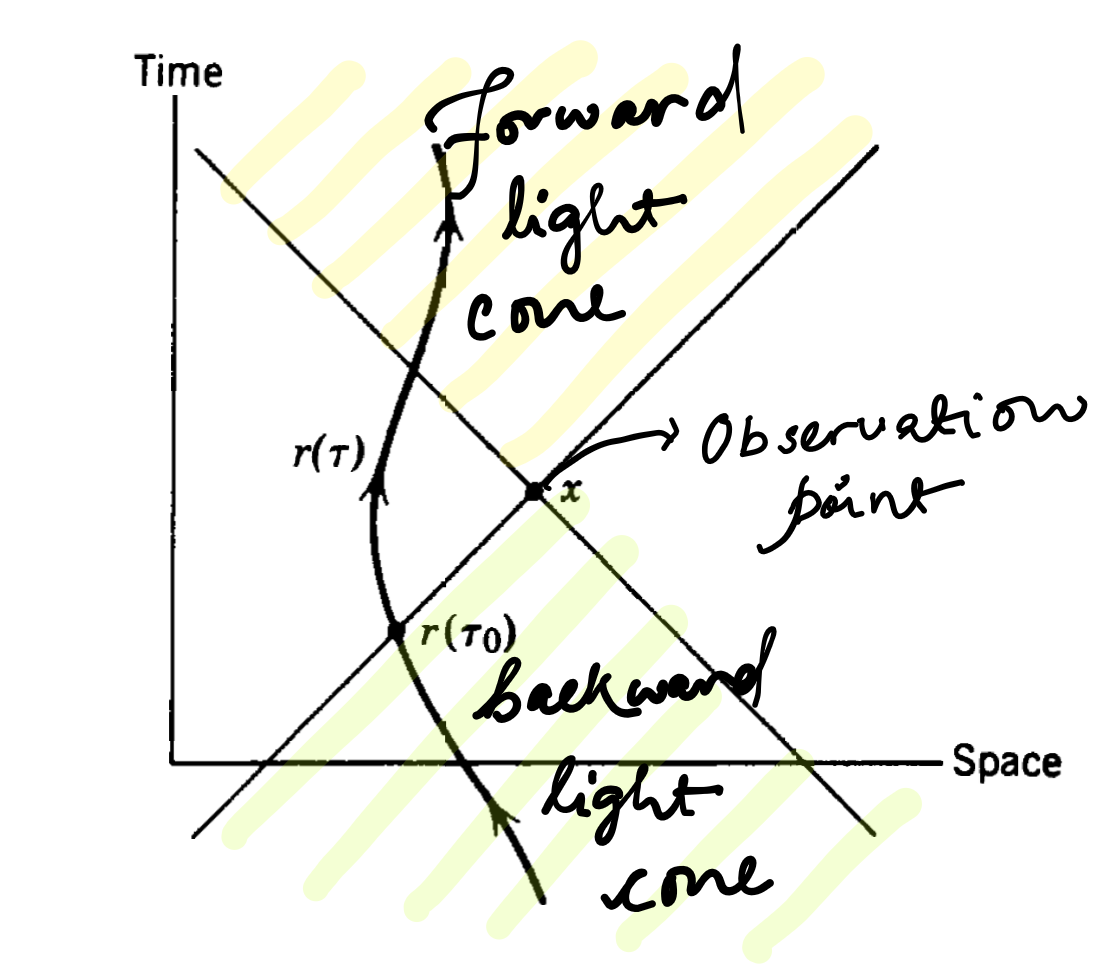
\includegraphics[width=0.7\linewidth]{lienardpot.png}
\label{radlineard}
\end{figure}
Now, focus on Fig. \ref{radlineard}. 
\begin{itemize}
\item Green Function is different from zero only on the backward lightcone of the observation point.
\item World line of the particle, $r(\tau)$, intersects the light cone at only two observation point, one earlier and one later than $x_0$.
\item Consequently in the earlier part, $r^\alpha(\tau_0)$ is the only part of the path that contributes to the field at $x^\alpha$.
\end{itemize}
Now, we know that
\begin{equation}\label{deltatau}
\delta[f(x)]=\sum_i \frac{\delta(x-x_i)}{|\cc{\pe{f}{x}}_{(x=x_i)}|}
\end{equation}
\textbf{Note:} Here, it was assumed that the zeros of $f(x)$ at $(x=x_i)$ are all linear.\\
and also we also need,
\begin{equation}
\frac{d}{d\tau}\rr{x-r(\tau)}^2 =2\rr{x-r(\tau)}_\beta \cc{-\frac{d r(\tau)}{d\tau}}^\beta=-2\rr{x-r(\tau)}_\beta V^\beta(\tau)
\end{equation}
which is evaluated at point $\tau=\tau_0$
\textbf{So, can we say that the motion of charged particle $r(\tau)$ is completely determined by the potential term?}

In our case, $\rr{x-r(\tau)}^2$ is function of $\tau$. In our case, only earlier point contributes to the path, so we consider only $r^\alpha(\tau_0)$ as zeros for \eqref{deltatau}.\\
Therefore, we have,
\begin{equation}\label{deltatau}
\delta([x-r(\tau)]^2)= \frac{\delta(x-r(\tau))}{|-2\rr{x-r(\tau)}_\beta V^\beta(\tau)|_{\tau=(\tau_0)}}
\end{equation}
Now, putting everything in \eqref{Vpotf}:
\begin{eqnarray*}
A^\alpha(x)=2e\int d\tau V^\alpha(\tau)\theta\rr{x_0-r_0(\tau)}\delta\rr{x-r(\tau)}^2\\
=2e\int d\tau V^\alpha(\tau)\theta\rr{x_0-r_0(\tau)}\frac{\delta(x-r(\tau))}{|-2\rr{x-r(\tau)}_\beta V^\beta(\tau)|_{\tau=(\tau_0)}}
\end{eqnarray*}
\begin{equation}
\implies A^\alpha(x)=\frac{e V^\alpha(\tau)}{\rr{x-r(\tau)}_\beta V^\beta(\tau)}|_{\tau=(\tau_0)}\\
\end{equation}
or,
\begin{equation}\label{liendardVpot}
\implies A^\alpha(x)=\frac{e V^\alpha(\tau)}{V . \rr{x-r(\tau)}}|_{\tau=(\tau_0)}
\end{equation}
where, \textbf{$\tau_0$ is defined by \eqref{lc} and Retardation requirement}. And \textbf{\eqref{liendardVpot} is called \tit{Lienard-Wiechert potentials}}.
We can further work on it. Now, Let:
\begin{equation}
x_0-r_0(\tau_0) = \mbf{|x_0-r_0(\tau_0)|} \equiv R
\end{equation}
Hence,
we can write:
\begin{eqnarray*}
\text{First we expand the individual 4 vector components of V.(x-r)}\\
V.(x-r)=V_0\rr{x_0-r_0(\tau_0)}-\mbf{V.\rr{x-r(\tau_0)}}
=\gamma cR-\gamma\mbf{v.n}R\\
\text{where, $\mbf{n}$ is a unit vector in the direction of}\\
\text{$\mbf{x-r(\tau)}$ and $\mbf{\beta=v(\tau)/c}$}\\
\implies \gamma c R(1-\mbf{\beta .n})
\end{eqnarray*}
Finally, we can wite the potential in the final form can be deomposed into components as
\begin{equation*}
 A^\alpha(x)=\frac{e V^\alpha(\tau)}{V . \rr{x-r(\tau)}}|_{\tau=(\tau_0)}
\end{equation*}

\section{Synchrotron Radiation: Basics}
Synchrotron radiation is emitted by charges spiralling in a magnetic field moving at relativistic speeds.\\
\textbf{Why is it important?}\\
Synchrotron has a broad frequency spectrum often corresponding to a million harmonics of the basic frequency of particle in motion.\\


A charged particle in constant magnetic field moves in a circular trajectory in plane perpendicular to $\mbf{B}$.\\
The angular velocity of such a particle with an energy E. If $v.\mbf{B}=0$, then particle moves in a circular path of radius
\begin{equation}
r_B=\frac{v}{\omega}=\frac{mcv}{qB}\gamma
\end{equation}
Before, we start with the business of Synchrotron. We first recapitulate the Synchrotron for non-relativistic electrons. \\

\begin{\cbox}
For non relativistic electrons accelerated by magnetic fields are said to emit cyclotron radiation. The radiation is at frequency of gyration $\omega=eB/m_ec$. 
\end{\cbox}
\textbf{For relativistic particles, this emission extends to higher frequencies and we call it Synchrotron Emission.}

\chapter{Continuum Radiation Processes}
\textbf{This Chapter is largely based on Klein Fetcher's book on galactic and intergalactic magnetic field, Chapter 2. The important point to note is, we will be doing the mathematical part behind radiation in our own time. This is a more applicative based study and less mathematical.}\\
\section{Introduction}
\textbf{Why is studying Sychrotron Radiation important?:}\\
We observe low frequency synchrotron radiation on galactic scales when relativistic electrons move in a magnetic field.\\ 
Studying synchrotron helps us to use it as a tool to trace magnetic fields in interstellar and intergalactic scales, by virtue of its \textbf{radiation spectrum and polarisation properties}.\\

\textbf{What is the issue with observing this low frequency radiation?}\\
The main point of concern is at radio frequency we not only observe the synchrotron radiation, it is contaminated by free-free radiation coming from \textbf{ionised HII regions} and \textbf{ionised medium of milky way} galaxy and other galaxy.\\

So it becomes important for us to know both \textbf{thermal(free-free)} and \textbf{non thermal(synchrotron)} part of energy so that we can extract out the non thermal component.\\
\begin{\cbox}
Free-Free is called thermal radiation because it results from an ensemble of particles with a \textbf{Maxwellian Energy Distribution}. On the other hand, energy distribution of synchrotron follows a power-law.
\end{\cbox}
\begin{\cbox}
Note point: In order to produce measurable Synchrotron radiation vs measurable thermal radiation, the number of relativistic particles required is less lower than the thermal ones. \textbf{Just because they are so energetic} 
\end{\cbox}
\section{Radiation of an Accelerated Electron}
\begin{figure}[th]
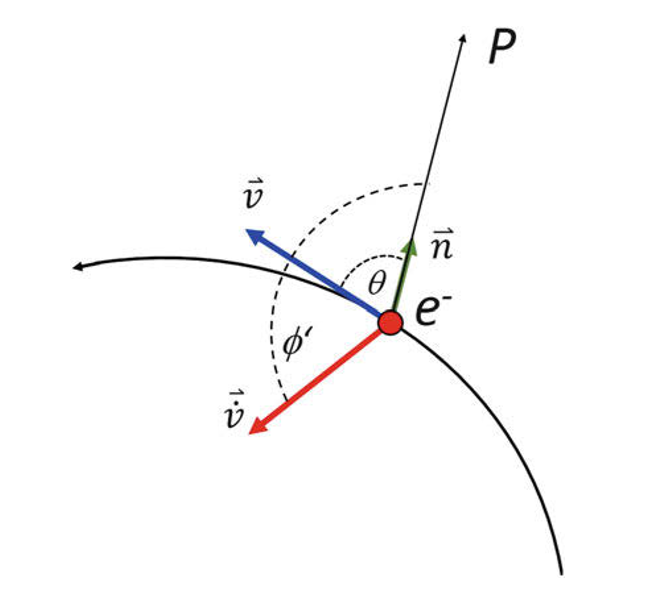
\includegraphics[scale=0.7]{singleprad.png}\label{singleprad}
\caption{Geometry for a moving charged particle as seen from the point P}
\end{figure}
\textbf{What is the electric field for an accelerated electron?}\\
So we have an accelerated electron as Fig. \ref{singleprad}. The velocity of the electron is $\vec{v}$ and the acceleration is $\vec{\dot{v}}$, as seen by observer at some point P. \textbf{Refer Chapter 14 Jackson} The electric field for such a particle is given as
\begin{equation}
\vec{E}=\cc{\frac{e}{c}}\cdot \frac{\vec{n}\times \rr{\cc{\vec{n}-\vec{\beta}}\times \vec{\dot{\beta}}\;}}{R\cc{1-\cos\theta \cdot \beta}^3}
\end{equation}
\begin{itemize}
\item $\vec{n}$ is unit vector pointing from the particle towards the observer.
\item $\beta=\frac{\vec{v}}{c}$ and $\vd{\beta}=\frac{\vd{v}}{c}$
\end{itemize}

\textbf{What is the flux of radiation and the power radiated?}\\
The flux of radiation is given by \textbf{Pontying Vector}
\begin{equation}
\vec{S}=\frac{c}{4\pi}\cdot \vec{E}\times\vec{B}=\frac{c}{4\pi}\cdot |\vec{E^2}|.\vec{n}
\end{equation}
The \textbf{power radiated into a unit solid angle per unit frequency and unit time} Units=[$Wstr^{-1}Hz^{-1}sec^{-1}$] is given by:
\begin{align}
\frac{dP(t)}{d\Omega}&=&|\vec{S}|\cdot(1-\beta \cos \theta)R^2\\
&=&\frac{e^2}{4 \pi c}\cdot \frac{|\vec{n}\times\rr{\vec{n}-\vec{\beta}}\times\vd{\beta}|^2}{(1-\beta \cdot \cos \theta)^5}
\end{align}
R being the distance between observer at point P and the electron.\\
The above equation will be used in the following case and form:
\begin{itemize}
\item $\beta<<1$ for  thermal radiation
\item $\beta\leq 1$ for non-thermal radiation
\end{itemize}
In order to find the power the above equation has to be modified over the $4\pi$ solid angle of the sphere. \textbf{Here, $\theta=\angle (\vec{v},\vec{n})$} and hence
\begin{equation*}
\cos \theta = \vec{n} \cdot \vec{\beta}
\end{equation*}
\begin{\cbox}
When measuring flux densities of radio sources, we can calculate their radio power or luminosity once we can determine this distance using standard astronomical techniques.Hence R is not relevant in the derivations that we shall work out below. It is just a matter of conversion from flux density to power or monochromatic luminosity, or from flux to total power or luminosity. So, converting for instance flux density $S_\nu$ to power $P_\nu$ then reads
\begin{equation*}
P_\nu=4 \pi R^2 S_\nu
\end{equation*}
Assuming the radio source emits isotropically.
\end{\cbox}
\textbf{Skipping the section on free-free Radiation for now!}
\section{Synchrotron Radiation}
\textbf{Why is Synchrotron radiation important? }\\
It basically serves as a diagnostic tool to trace magnetic fields in the ISM and IGM. \\
\textbf{How are the electrons in IGM and ISM are relativistically energised?}\\
\begin{itemize}
\item Electrons are energised in ISM by the shock waves produced during supernovae explosions\\
\item and energised due to AGN activity, by galactic wakes\fn{it is the hypersonic flow of intergalactic gas past a galaxy. \textbf{not sure!!} } and by merging of galaxies for the case of IGM.
\end{itemize}
\textbf{A brief overview:}
\begin{itemize}
\item Relativistic electrons in magnetic field experience Lorentz force.
\item This force makes the particles move in helical motion.
\item This accelerated helical motion leads to synchrotron radiation.
\item This radiation has a characteristics frequency spectrum and is \textbf{partially polarised.}
\end{itemize}
\begin{\cbox}
 galaxies and AGN exhibit synchrotron radiation as soon as they come into existence, a mere few hundred million years after the Big Bang. In fact, the distribution of faint(hence distant)radio sources is characterised by near isotropy,in accord with the cosmological principle. The bulk of these sources are AGN, which may produce Doppler boosting, which renders them detectable out to cosmological distances. 
\end{\cbox}
Another important observable is Faraday Rotation is \textbf{Faraday Rotation} - It allows us to estimate \textbf{Magnetic field strength} and \textbf{and their orientation} (towards and away from us) in the medium towards the radio source.
\subsection{Radiation from a single electron}
So as we already know power radiated from a single relativistic particle into a unit solid angle per unit frequency and per unit time is given by \eqref{eq:rel1particle}
\begin{figure}[h!]
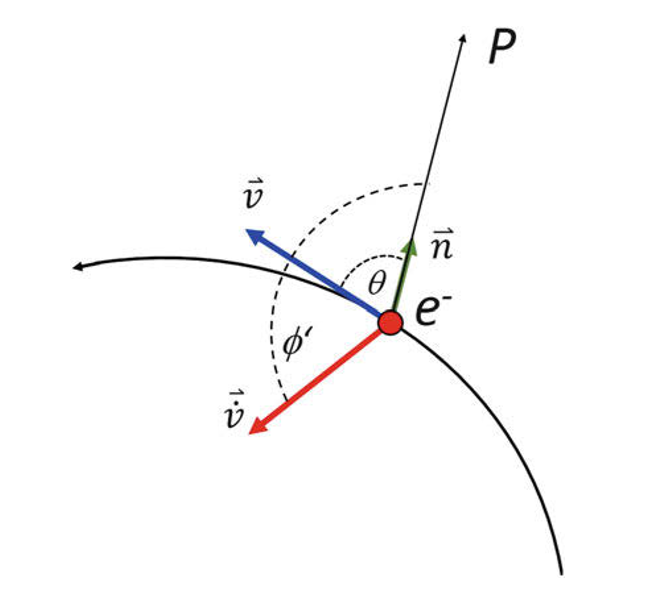
\includegraphics[height=4cm,width=9cm]{singleprad.png}
\caption{Geometry for a moving charged particle as seen from the point P}
\end{figure}

\begin{equation}\label{eq:rel1particle}
\de{P}{\Omega}=\frac{e^2}{4 \pi c} \cdot \frac{|\vec{n}\times \rr{(\vec{n}-\vec{\beta})\times\dot{\vec{\beta}}}|^2}{(1- \vec{n}\cdot \vec{\beta})^5}
\end{equation}
\begin{itemize}
\item $\vec{n}$ is unit vector pointing from the particle towards the observer.
\item $\beta=\frac{\vec{v}}{c}$ and $\vd{\beta}=\frac{\vd{v}}{c}$
\end{itemize}
When dealing with relativistic particles, we study two cases of the direction of $\vd{\beta}$ and $\beta$.
\begin{enumerate}
\item \tbf{LINEAR ACCELERATOR or }($\vd{\beta} \parallel \beta$):
Then we have the power radiated derived from \eqref{eq:rel1particle} to be :
\begin{equation}\label{eq:rel1particlelin}
\de{P}{\Omega}=\frac{e^2 \dot{v^2}}{4 \pi c} \cdot \frac{\sin^2 \theta}{(1- \cos \theta \beta)^5}
\end{equation}
\tbf{It is to be noted that:the radiation pattern has a strong dependence on the angle  and on the particle speed}. Refer to book to check out how $\beta$ influences radiation pattern. \tbf{\tit{What do we mean when we say radiation pattern, what are we plotting?}}.
The reason for strong dependence of value of $\beta$ on radiation pattern is because the maximum power radiated depends on $\gamma$ i.e.
\begin{equation}
\de{P}{\Omega}(\theta_{max}) \sim \gamma^8
\end{equation}
where,
\begin{equation}
\cos \theta_{max}=\frac{1}{3 \beta}\cc{\sqrt{1+15 \beta^2}-1}
\end{equation}
The above equations can be obtained by maximizing equation \eqref{eq:rel1particlelin} with respect to $\theta$ and then substituting  back in \eqref{eq:rel1particlelin} and $\theta_{max}=\frac{1}{2\gamma}$ i.e. is the maximum power is radiated when $\theta$ is very small and photons are emitted in the direction of acceleration.
\begin{\cbox}
The strong dependence on the Lorentz factor is called 'relativistic boosting' or 'beaming', meaning that a charged particle moving with relativistic speed emits essentially its whole radiation in the forward direction. 
\end{\cbox} 

The total radiation of the relativistic particle is given by the integration:
\begin{eqnarray*}
P(t)=\int^{2\pi} _{0} \int^{\pi} _{0} \de{P}{\Omega} d\Omega \\
\implies P(t)=\int^{2\pi} _{0} \int^{\pi} _{0} \frac{e^2 \dot{v^2}}{4 \pi c} \cdot \frac{\sin^2 \theta}{(1- \cos \theta \beta)^5} \sin^2 \theta d\theta d\phi \\
\implies P(t)= \frac{e^2 \dot{v^2}}{2 c} \int^{\pi} _{0}  \frac{\sin^2 \theta}{(1- \cos \theta \beta)^5} \sin^2 \theta d\theta \\
\implies P(t)=\frac{2}{3}\cdot \frac{e^2 \dot{v^2}}{c^3} \cdot \gamma^6
\end{eqnarray*}

\item \tbf{Transverse or CYCLOTRON ACCELERATOR or SYNCHROTRON }($\vd{\beta} \perp \beta$): Check Figure \ref{figtrac}. The geometry of and various angle required are given in right hand cartoon and the left hand cartoon refers to the same particle moving in interstellar magnetic field. 
\begin{figure}[h!]\label{figtrac}
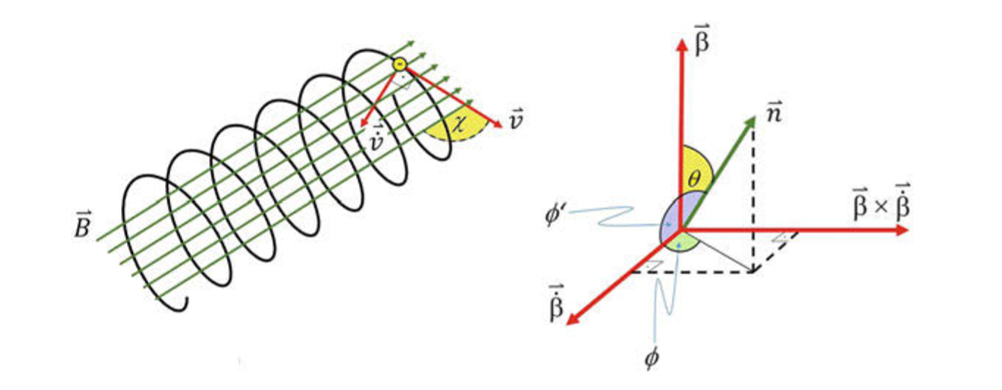
\includegraphics[scale=1]{figtrac}
\caption{ Illustration of the various angles used in describing the transverse acceleration of a relativistic electron in a magnetic field}
\end{figure}
\end{enumerate}
\textbf{Define Pitch angle:}\\
Pitch angle is the motion of particle is inclined to the magnetic field vector. In Figure \ref{figtrac} $\chi$ is the \textbf{pitch angle}.\\

 Now the, particle experiences \textbf{Lorentz force} and $\vec{\beta} \perp \vd{\beta}$ and 
\begin{eqnarray}
\de{P}{\Omega}=\frac{e^2}{4 \pi c} \cdot \frac{|\vec{n}\times \rr{(\vec{n}-\vec{\beta})\times\dot{\vec{\beta}}}|^2}{(1- \vec{n}\cdot \vec{\beta})^5}
\implies \de{P}{\Omega}=\frac{e^2 \dot{v^2}}{4 \pi c^3} \cdot \frac{1-\frac{\sin^2 \theta \cos^2 \phi }{\gamma^2(1-\beta \cos \theta)^2}}{(1-\beta \cos \theta)^3}
\end{eqnarray}
\textbf{As in case of the linear accelerator, the relativistic motion causes a relativistic aberration of the radiation of the charged particle, i.e. a strong distortion of the radiation pattern. check Figure \ref{figtracpa}}
\begin{figure}[h!]\label{figtracpa}
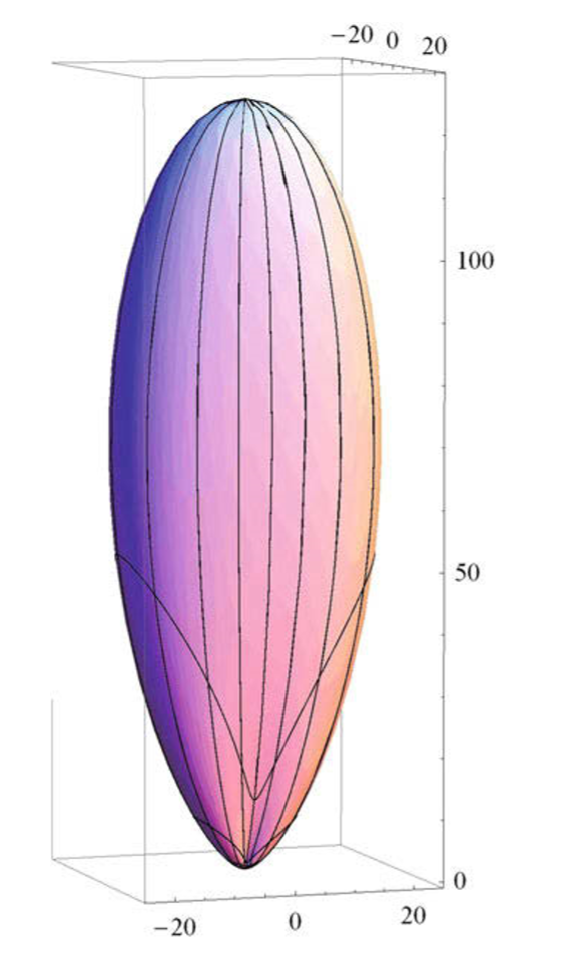
\includegraphics[scale=1]{figtracpa.png}
\caption{Radiation pattern of the transversely accelerated electron ($\beta$:0.8)}
\end{figure}
\textbf{Its main lobe can be shown to have a half-power width that is inversely proportional to the Lorentz factor 1=$1/\gamma$ at half-maximum} or 
\begin{equation}
\theta_{HP}\approx 1/\gamma =\frac{m_0c^2}{E^2}
\end{equation}
Note:The half-power width is the angular width of the radiation  pattern at which the power has dropped to half its maximum value.\\
\textbf{As in case of the transverse accelerator, the radiated power has a strong dependence on the Lorentz factor:
\begin{equation}
\de{P}{\Omega} \sim \dot{v^2}\gamma^6
\end{equation}
and
\begin{equation}
P(t)=\int^{2 \pi} _{0}\int^{ \pi} _{0} \de{P}{\Omega} d\Omega \sim \dot{v^2}\gamma^4
\end{equation}
}

Now, we try to calculate the Larmor Circle and at the end of it you would understand why we need it at all:\\
Now, the equation of motion a charged particle in magnetic field is given by
\begin{equation}
m\vd{v}=m\cdot (\vec{v}\times \vec{\omega_L})=\frac{-e}{c}(\vec{v}\times \vec{B})
\end{equation}
Let us consider the pitch angle, $\chi=90^circ$ i.e. the particle motion is perpendicular to the magnetic field.Hence,
\begin{eqnarray}
m\omega^2_Lr_L=m\cdot \frac{v^2}{r_L}=\frac{e}{c} \cdot vB
\implies m\frac{v}{r_L}=\frac{e}{c} B\\
\implies \omega_L=\frac{eB}{mc}
\end{eqnarray}
Now for a relativistic particle we know, $m=\gamma m_0$, since $E=mc^2=\gamma m_0c^2$. Therefore,
\begin{equation}
\omega_L=\frac{eB}{mc}
\end{equation}
and the larmor radius for $v\approx c$ is
\begin{equation}
r_L=\frac{v}{\omega_L}=\frac{m_0vc}{eB}\cdot \gamma\approx \frac{m_0c^2}{eB}\cdot \gamma =\frac{E}{eB}
\end{equation}
or in general,
\begin{\cbox}
\begin{equation}
r_L=\frac{E}{eB}\sin \chi
\end{equation}
We realise that the Larmor radius does not depend on the mass of the particle, but just on its energy (and on the magnetic- field strength). 
\end{\cbox}
Now, for a $\gamma=1$ and a magnetic field of $B=10\mu G$ we have a frequency of 28Hz. 
\textbf{Now, the question may be asked that how can we observe such particles in radio regime? The answer to this question is in}

\begin{\cbox}
\textbf{what we have found is the power emitted by the relativistic particle in the direction of observer, but we need to make a frame transition to observer's frame if we want to obtain power spectrum seen by the observer}
\end{\cbox}
Therefore, the way the observer observes the radiation from electron is is by calculating the time dependence of radiation as seen by the observer.\\
Now, in order to calculate the radiation spectrum \textbf{ we perform a Fourier analysis of the time-dependent radiation power of single particles,then 'fold in' their energy spectrum and then calculate the emissivity.} The frequency of the emitted pulses of the gyrating relativistic electrons \textbf{ corresponds to the inverse of the time that the radiation pattern needs to sweep across the observer}.
Therefore, we can visualize the radiation emitted by the particle as given in Fig. \ref{figobsrad}
\begin{figure}\label{figobsrad}
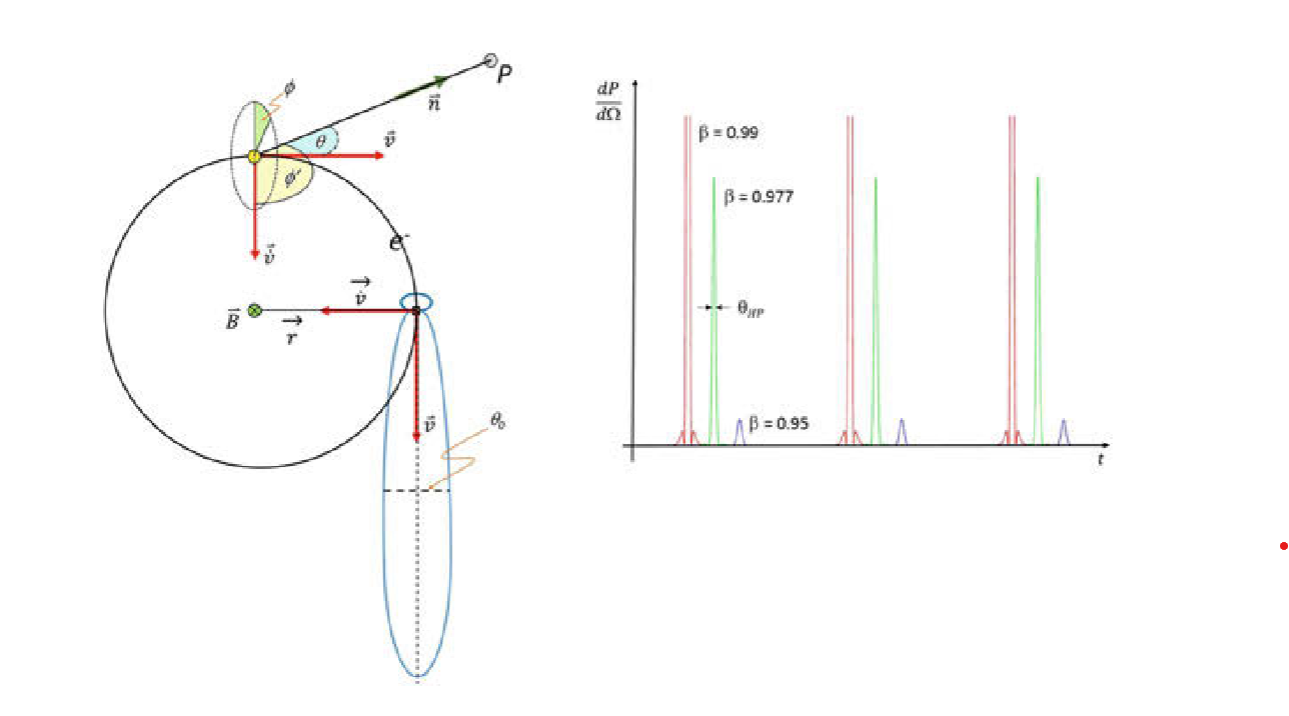
\includegraphics[scale=1]{figobsrad.png}
\end{figure}
\textbf{Now, how long does the pulse last in particle's frame of reference:}\\
The duration of the pulse in the particle's frame of reference is equal to:
\begin{equation}
\Delta t =\frac{r_L\theta_{HP}}{v}\approx \frac{r_L \theta_{HP}}{c}
\end{equation}
and since, $r_L \approx \frac{Ee}{B}$ and $\theta_{HP}\approx \frac{1}{\gamma}$, we find 
\begin{equation}
\Delta t =\frac{m_0 c}{e B}
\end{equation}
Our next order of business would be transforming frames from particles to observer i.e. from t frame to $t^\prime$.\\
The transformation is shown in Figure \ref{figtrans}. What we need to account is the motion of particle when it emitted the pulse of duration $\Delta t$. Therefore our transformation time is given as 

\begin{figure}[h!]\label{figtrans}
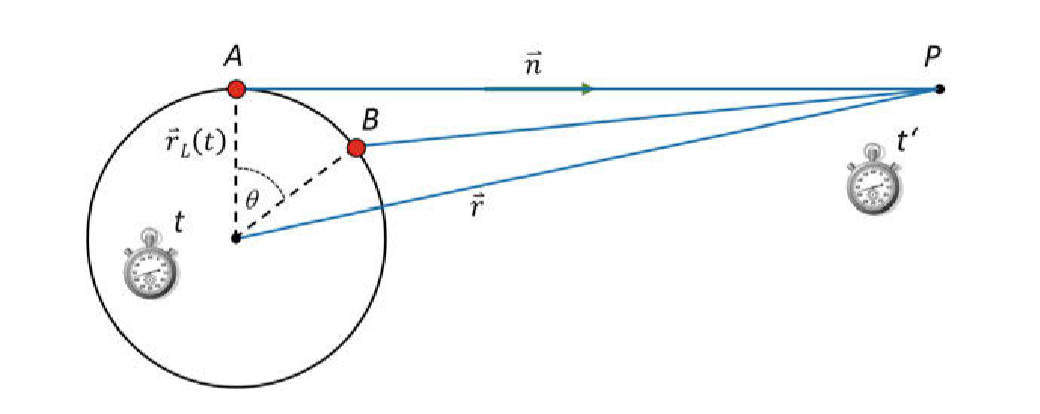
\includegraphics[width=\linewidth]{figtrans.png}
\caption{geometry of the transformation from the particle's to the observer's reference frame}
\end{figure}
\begin{equation}
t^\prime=t+\frac{|\vec{r}-\vec{r_L(t)}|}{c}
\end{equation}
Now, the rate of change of time in one frame to another is given as follows:
\begin{eqnarray*}
t^\prime=t+\frac{|\vec{r}-\vec{r_L(t)}|}{c}\\
\implies t^\prime=t+\frac{\cc{\cc{|\vec{r}-\vec{r_L(t)}|}^2}^{1/2}}{c}\\
\implies \de{t^\prime}{t}=1-\frac{\vec{r}-\vec{r_L(t)}}{|\vec{r}-\vec{r_L(t)}|}\cdot \de{\vec{r_L(t)}}{t}\\
\implies \de{t^\prime}{t}=1-\frac{\vec{n}\cdot \vec{v}}{c}=1-\beta \cdot \cos \theta_{HP}\\
\tx{I think $\theta_{HP}$ is the average value of angle between $\vec{n}$ and $\vec{v}$}\\
\tx{and, for small angles}\\
\implies \de{t^\prime}{t}=1-\beta \cdot \sqrt{1- \theta^2_{HP}} \\
\implies \de{t^\prime}{t}=1-\beta \cdot \sqrt{1- \frac{1}{\gamma^2}} \\
\implies \de{t^\prime}{t}=1-\beta^2 =\frac{1}{\gamma^2} \\
\end{eqnarray*}
\begin{\cbox}
\begin{equation}
\Delta t^\prime =\frac{\Delta t }{\gamma^2}
\end{equation}

\end{\cbox}
Now, Remember the argument of particle emitting at frequency 28Hz at $B=10\mu G$, for $\gamma=2000$, the frequency spectrum is shifted towards a $\gamma^2$ higher range and that would be around $\nu=700MHz$.\\
Now we define \tbf{a critical frequency} and the purpose of this being \tbf{the particles produce a significant power at this frequency}. given as $\omega_c =2 \pi \nu_c$. Even though $\omega_c$ has different definitions, we will use one by Schwinger 
\begin{equation}
\omega_c\equiv \frac{1}{\frac{2}{3}\Delta t^\prime}
\end{equation}
and substituting the value of $\Delta t$ here we get
\begin{\cbox}
\begin{equation}
\nu_c=\frac{3}{4 \pi}\cdot \frac{e B_{\perp}}{m_0c}\cdot \gamma^2
\end{equation}
Here, $B_{\perp}=B \cdot \sin \chi$. is the component of the magnetic field perpendicular to the line-of-sight.
\end{\cbox}
\textbf{So far so good, we have considered the synchrotron emission from particles composed of only electrons. What about protons? Evidently, The cosmic-ray (CR) energy spectrum observed near earth exhibits $\sim 100$ times more protons than electrons (at the same energy).}\\
Here, we now check for the contribution of protons:\\
So, we know,
\begin{equation}
\nu_c=\frac{3}{4 \pi}\cdot \frac{e B_{\perp}}{m_0c}\cdot \gamma^2
\end{equation}
We substitute $\gamma= \frac{E}{m_0c^2}$. 
\textbf{This tells us a crucial fact, $\nu_c$ depends on the mass of the radiating particle like $m^{-3}$}. And, we can find that
\begin{equation}
\cc{\frac{m_p}{m_e}}^{-3}=1.6 \cdot 10^{-10}
\end{equation}
and hence the frequency for proton relative to electron would be around
\begin{equation}
\cc{\frac{\nu_{c,p}}{\nu_{c,e^{-1}}}}=1.6 \cdot 10^{-10}
\end{equation}
\textbf{Put differently, we can calculate how much more kinetic energy a proton must have in order to radiate at the same frequency as the electron.}
\begin{equation}
E_p=\cc{\frac{m_p}{m_e}}^{3/2}\cdot E_e =8\cdot 10^4 E_e
\end{equation}
\textbf{Hence, even the ratio of number densities measured in the CR energy spectrum of $np/ne \approx 100$ does not help. In fact, as we shall see later, \tit{relativistic protons are much more long-lived, owing to their very low radiation losses. They may remain relativistic for more than a Hubble time, while electrons become non-relativistic within less than 100 Myr}}\\
Remember the power of the time dependent radiated power into a unit solid angle per unit frequency and per unit time is
\begin{align}
\frac{dP(t)}{d\Omega}&=&\frac{e^2}{4 \pi c}\cdot \frac{|\vec{n}\times\rr{\vec{n}-\vec{\beta}}\times\vd{\beta}|^2}{(1-\beta \cdot \cos \theta)^5}
\end{align}
For, small angle $\theta$ and large Lorentz factors $\gamma$\textbf{Note: I have not done this calculation yet.}
\begin{equation}
frac{dP(t)}{d\Omega}=\frac{2}{\pi}\;\frac{e^2 \dot{v}^2}{c^3} \gamma^6\cdot \frac{1}{(1+\gamma^2 \theta^2)^3}\cdot \rr{1-\frac{4 \gamma^2 \theta^2 \cos^2 \phi}{(1+\gamma^2\theta^2)^2}}
\end{equation}
and, upon integration over solid angle it becomes
\begin{equation}\label{eq:timeP}
P(t)=\int^{2 \pi}_0 \int^{\pi}_0 \de{P}{\Omega}d\Omega=\frac{2}{3}\frac{e^2\dot{v}^2}{c^3}\cdot\gamma^4
\end{equation}
Now, what we do is the \tbf{Fourier analysis of time-dependent radiated power} for the small angle approximation [\textbf{Done by schwinger}]:
\begin{equation}
P(\nu)=\frac{\sqrt{3}e^3}{m_0 c^2} \cdot B_{\perp} \cdot F\cc{\frac{\nu}{\nu_c}}
\end{equation}
where
\begin{equation}\label{eq:freqP}
F\cc{\frac{\nu}{\nu_c}}=\frac{\nu}{\nu_c}\cdot \int^\infty_{\nu/\nu_c} K_{5/3}(x)dx
\end{equation}
\textbf{The function $F\cc{\frac{\nu}{\nu_c}}$ is the Airy integral of the modified Bessel Function $K_{5/3}(x)$}. Th Wallis approximation renders us the following important result
\begin{\cbox}

\begin{equation}
F\cc{\frac{\nu}{\nu_c}}=1.78 \cc{\frac{\nu}{\nu_c}}^{0.3} \cdot e^{-\frac{\nu}{\nu_c}} 
\end{equation}
\end{\cbox}
Using \eqref{eq:timeP} and \eqref{eq:freqP} we can plot for various values of $\gamma$ as given in Figure \ref{figfour}

\begin{figure}\label{figfour}
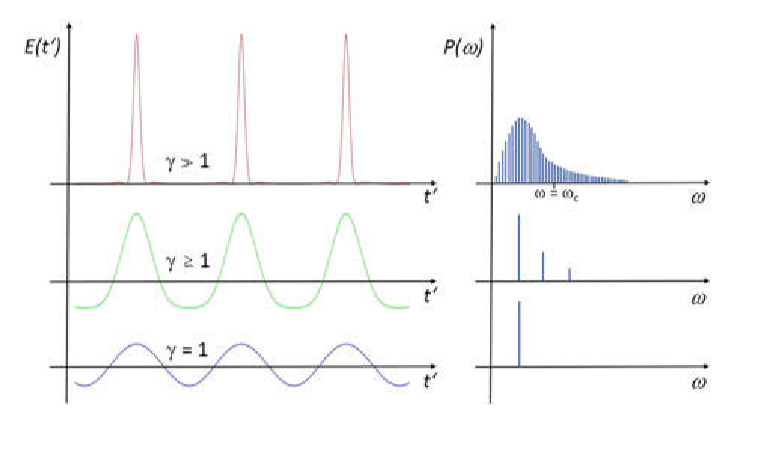
\includegraphics[scale=1]{figfour.png}
\caption{Sketch of the time dependence of the synchrotron pulses and their radiation spectra}
\end{figure}

\subsection{Synchrotron Radiation from Relativistic Electrons with an Energy Spectrum}
Now, if we need to measure the radiation coming in from a bunch of particles we would need to know the energy spectrum of the bunch of charges. The CR shower on the atmosphere has been observed and identified to follow as power lay given as given as
\begin{equation}
N(E)dE=A\cdot E^{-g}dE
\end{equation}
and plotted in Figure \ref{figepower} which shows the measured energy spectrum near earth.
\begin{figure}\label{figepower}
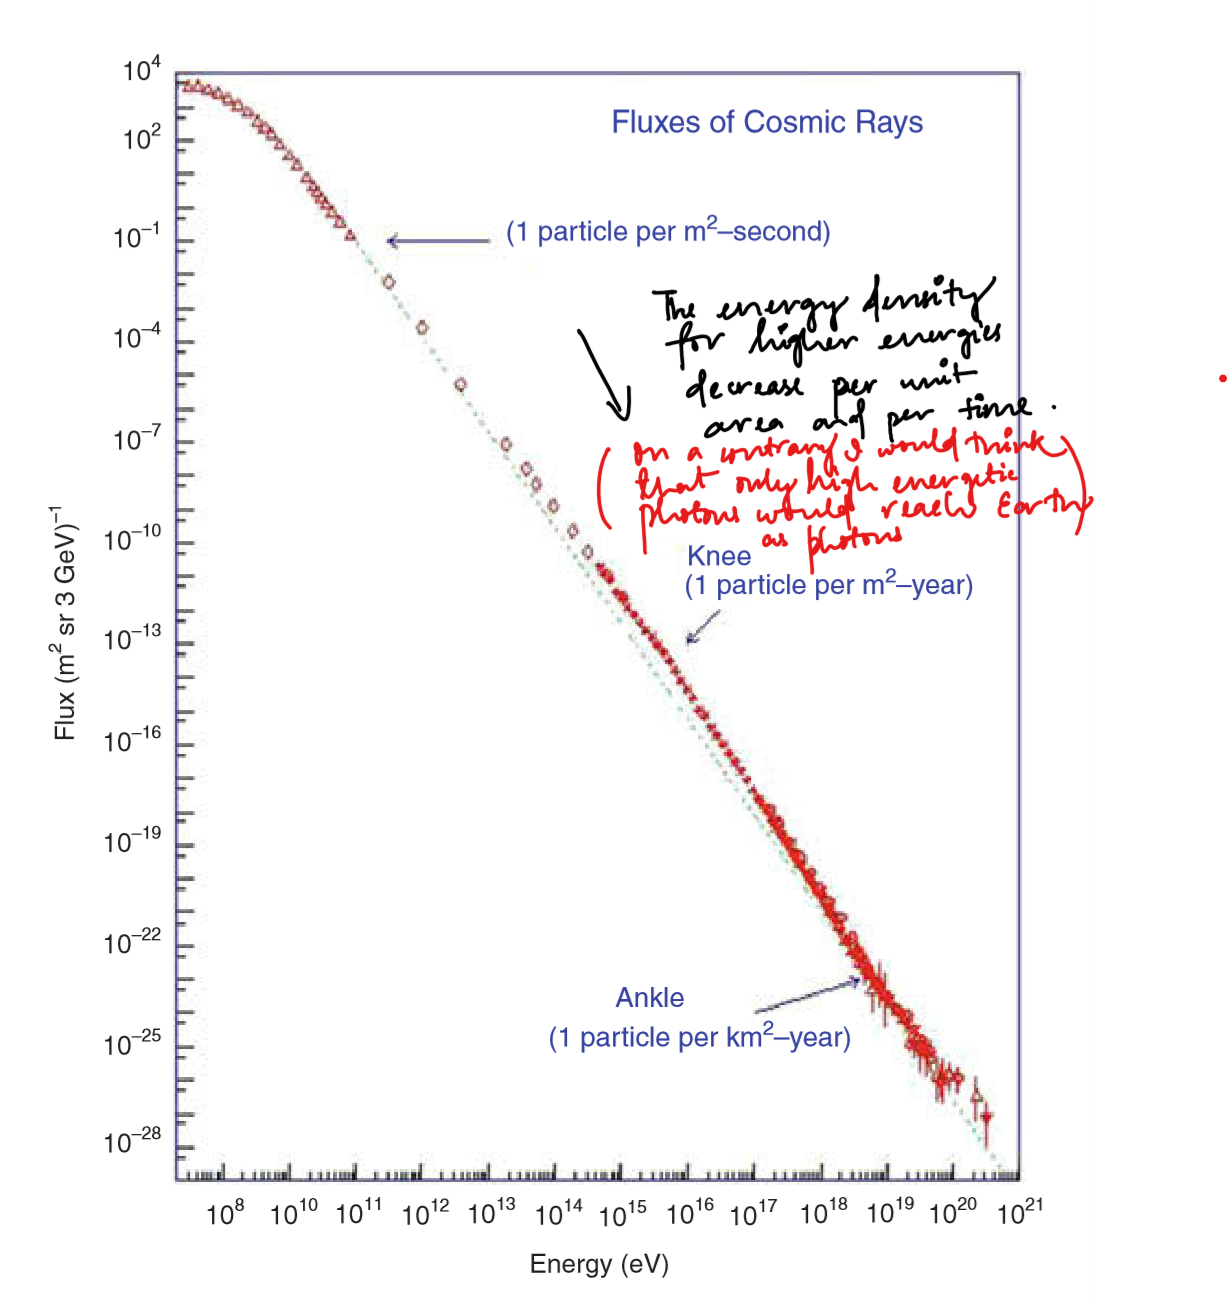
\includegraphics[scale=1]{figepower.png}
\end{figure}
\begin{itemize}
\item A is a constant. Representing the local number density of relativistic particles per energy interval.
\item g is the power law index , \textbf{generally g=2.4}
\end{itemize}
Coming back to Figure \ref{figepower}:
\begin{itemize}
\item ($\leq 1GeV - 10's\;\;GeV$): Represents energies of particles emitting synchrotron
\item  measured spectrum is strongly modulated by the solar wind below a few GeV, which explains the deviation from the power-law there. Hence, nothing is known about the shape of the spectrum at the lowest CR energies. 
\item  At the highest energies, there are changes in the spectrum called 'knee' (at $\geq 10^{15}$ eV) and 'ankle' (at $\geq 10^{18}$ eV).
\item  The particles with the highest recorded energies($\geq 10^{20}$ eV, so-called ultra-high energy cosmic rays, or UHECR) are a real enigma, their origin being totally unknown.

\end{itemize}
Now, the intensity of emission is given through the emissivity equation:
\begin{equation}
4 \pi \epsilon_\nu=\int^{E_2}_{E_1}P(\nu)\cdot N(E)dE
\end{equation}
\textbf{Assuming that there is no background radiation, the radiation transport equation yields the intensity from the brightness and the source function}
\begin{equation}
I_\nu=S_\nu(T)\cdot (1-\exp^{-\tau_\nu}) \approx S_\nu(T)\cdot \tau_\nu
\end{equation}
for small values of $\tau_\nu$. we expect the medium to more or less transparent to the observed frequency but \textbf{should the $\tau_\nu$ not be tending more toward infinity. then why do we assume that the $\tau_\nu$ is small?}.\\
From Kirchoff's law we have \textbf{Look into this too}
\begin{equation}
S_\nu(T)=\frac{\epsilon_\nu}{\chi_\nu}
\end{equation}
result in
\begin{equation}
I_\nu=\int^{s_0}_0\epsilon_\nu ds
\end{equation}
and hence
\begin{equation}
I_\nu=\frac{1}{4\pi}\int^{s_0}_0 \int^{\infty}_0 P(\nu) N(E)dEds
\end{equation}
\textbf{check about above definition I am not so sure!!!!}\\
The units of brightness or intensity is given as $\rr{erg\;\;s^{-1}\;\;cm^{-2}\;\;Hz^{-1}\;\;sr^{-1}}$.\\
\tbf{\tit{ Let us assume for simplicity that neither the power $P(\nu)$ nor does the energy spectrum depends on the location.}}\\
i.e. $dP/ds=0$ and $dN/ds=0$.\\
Using the equations of Power in frequency domain and energy spectrum we have
\begin{equation}
I_\nu=\frac{s_0}{4\pi}\cdot \frac{\sqrt{3}e^3}{m_0c^2}\cdot B_{\perp} A \cdot \int^{\infty}_0 F\cc{\frac{\nu}{\nu_c}}E^{-g}dE
\end{equation}
\textbf{$s_0$ being the total path length}.\\
When push in Waalis approximation
\begin{equation}
I_\nu=\frac{s_0}{4\pi}\cdot \frac{\sqrt{3}e^3}{m_0c^2}\cdot B_{\perp} A \cdot 1.78 \cdot \int^{\infty}_0 \cc{\frac{\nu}{\nu_c}}^{0.3} \dot e^{-\nu/\nu_c}E^{-g}dE
\end{equation}
Let's do some assignments for abstraction:
\begin{eqnarray*}
C\equiv 1.78  \frac{\sqrt{3}e^3}{4 \pi m_0c^2}=3.32 \times 10^{-23}esu^3 erg^{-1}\\
\nu_c=\frac{3}{4\pi}\cdot\frac{eB_{\perp}}{m_0^3c^5}\cdot E^2\equiv \eta B_{\perp} E^2\\
\eta=6.26 \times 10^{18}s^4g^{-5/2}cm^{-7/2}
\end{eqnarray*}
We also make use of substitution
\begin{equation}
\sqrt{\frac{\nu_c}{\nu}}\equiv x =\cc{\frac{\eta \cdot \beta}{\nu}}^{1/2}\cdot E
\end{equation}
i.e.
\begin{equation}
dE=\cc{\frac{\nu}{\eta B}}^{1/2}dx
\end{equation}
To be derived:\\
The expression for intensity is given as
\begin{equation}
I_\nu=s_0 C A \eta^{\frac{g-1}{2}}B_{\perp}^{\frac{g+1}{2}}\nu^{\frac{-g+1}{2}}\int^\infty_0 x^{-(g+0.6)}e^{-\frac{1}{^2}}dx
\end{equation}
\begin{\cbox}
Not only for Milky way but even for external galaxies h=2.4
\end{\cbox}
Therefore with
\begin{equation}
\frac{1}{x^2}=u \implies \frac{-2}{x^3}dx=du
\end{equation}
we have
\begin{equation}
\int^\infty_0x^{-3}\cdot e^{-\frac{1}{x^2}}dx=\frac{1}{2}\int^\infty_0 e^{-u}du=\frac{1}{2}
\end{equation}
and using $g=2.4$ we finally have
\begin{\cbox}
\begin{equation}
I_\nu=2.4 \cdot 10^{-10}\cc{\frac{s_0}{cm}}\cc{\frac{A}{erg^{1.4}cm^{-3}}}\cc{\frac{B_\perp}{G}}^{1.7}\cc{\frac{\nu}{Hz}}^{-0.7}
\end{equation}
\end{\cbox}
which has the dimensions of $\rr{erg\;\;s^{-1}\;\;cm^{-2}\;\;Hz^{-1}\;\;sr^{-1}}$.\\
let us look into some numbers first some number crunching, \\
The value of A $=8.2 \times 10^{-17}erf^{1.4}cm^{-3}$ close to earth, this is true. But we take it constant over a line of sight of 10Kpc, then the magnetic field would expect synchrotron intensity as
\begin{equation}
I_\nu \approx 10^{18} erg s^{-1} cm^{-2} Hx^{-1} sr^{-1}
\end{equation} 
at an observing frequency of $\nu =1GHz$.\\
In general if
\begin{\cbox}
The energy spectrum is given by:
\begin{equation}
N(E)dE\sim E^{-g}dE
\end{equation}
then we have
\begin{equation}
I_\nu \sim B_{\perp}^{1+\alpha}\cdot \nu^{-\alpha}
\end{equation}
where $\alpha$ is the spectral index . The spectral index related to the power law index  $g$ as 
\begin{equation}
\alpha=\frac{g-1}{2}
\end{equation}
For ISM, g=2.4 and $\alpha=0.7$.
\end{\cbox}
\textbf{ The synchrotron spectrum steepens in regions of lacking energy supply , while in the vicinity of star-forming regions in which stellar winds and supernovae cause turbulence and (re-)accelerate the particles. What is happening in computing I
is that for each electron the radiation spectrum P($\nu$) of the single particle is successively multiplied by the 'particles' number density for each energy. The integration over the whole energy range then yields the frequency spectrum. In the log-log plot this means that we have to add (logarithmically) the 'weighting functions', given by N(E). \tit{If the energy spectrum has a cut-off at some energy $E_{max}$, the spectrum will fall off exponentially beyond the corresponding critical frequency}}.
\begin{equation}
\nu_c=\frac{3}{4 \pi}\cdot \frac{e. B_{\perp}}{m_0c}\cdot \gamma^2_{max}
\end{equation}
Now, we show an illustration for the cut off frequency and single electron spectrum plot in Figure. \ref{figsyn}
\begin{figure}\label{figsyn}
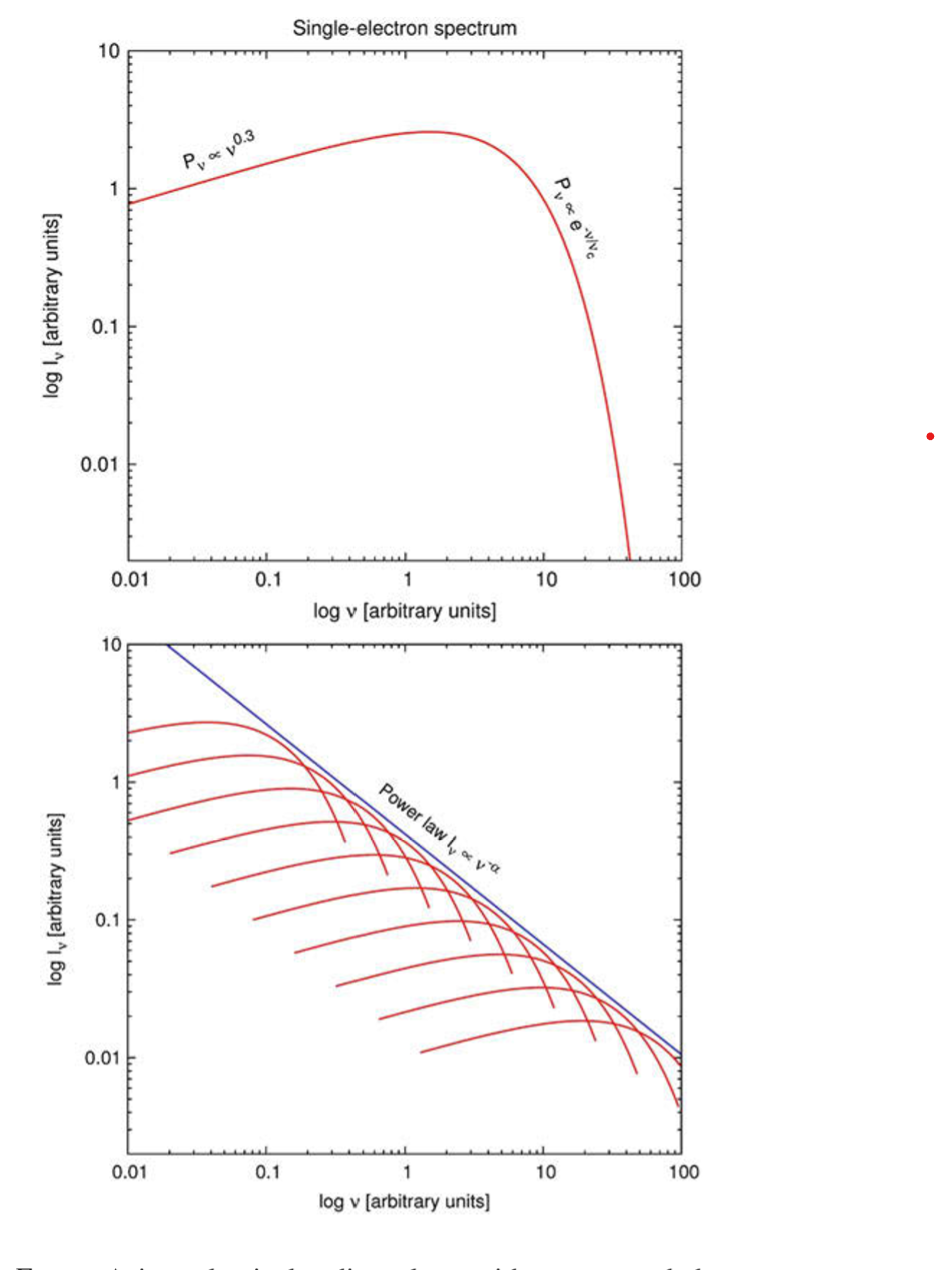
\includegraphics[scale=1]{figsyn.png}
\end{figure}
\chapter{Diffuse Radio Emission from Galaxy Clusters}
\textbf{This work is largely based on R.J.  Van Weeren's review paper with the same title}
\section{Abstract}
With increased detection of galaxy clusters there has been increased identification of the diffuse extended radio sources. \textbf{Note point: These sources may not be individually linked to host cluster galaxies.}And the radio emission from these sources reveal the presence of \textbf{cosmic rays and magnetic fields in the intra-cluster medium (ICM)}\\
\textbf{What comprises of this intra-cluster medium?}\\
\textbf{What are cosmic rays and why are they important at all?}
The diffuse cluster radio sources can be classified as:
\begin{itemize}
\item Radio Halos: They can be further classified as:
\begin{itemize}
\item Giant halos
\item Mini halosa
\item Ans possible intermediate sources
\end{itemize}
\textbf{Where do you find these halos and how does their brightness vary?}\\
 Halos are generally positioned at cluster center and their brightness approximately follows the distribution of the thermal ICM.\\
 \textbf{How are halos formed at cluster center and why is the brightness following the distribution of the thermal ICM?}\\
\item Cluster Radio Shocks(Relics): These are generally found in Cluster's periphery.\\
\textbf{Again, here it becomes important to know how are the relics formed? what do we know about them?}\\
\textbf{\textit{One very crucial property here is they are tracer for merger induced shock waves!!}}
\item Revived AGN fossil plasma sources:\\
\textbf{Among other sources, how do you identify Revived fossil plasma sources?}\\
Ans. \begin{itemize}
\item They have steep radio spectra. I guess in the intensity vs frequency graph, it rises very fast.
\item They have irregular morphologies
\end{itemize}
\end{itemize}
\textbf{What will you study here?}\\
\begin{itemize}
\item We will have an overview of recent results regarding properties of this diffused sources.
\item We will discuss, the resulting implications for the underlying physical acceleration processes that operate in the ICM.
\item we will discuss, the role of relativistic fossil plasma and the properties of ICM shocks and magnetic fields.
\end{itemize}
\newpage
\section{Introduction}
When we talk about scales in universe, galaxy clusters are \textbf{largest virialized objects} objects in the universe. $M_{cluster}=\sim 10^{15} M_\odot$. Located between clusters, elongated filaments of galaxies, form even larger unbound structures, making up the cosmic web. These filaments span the regions between clusters. 


\textbf{Galaxy clusters are located at the nodes of filaments, like spiders in the cosmic web.}\\
\textbf{What is ICM? What is its emission form like?}\\
Ans. Clusters may contain up to several thousands of galaxies. However, the galaxies comprise \textbf{of only $1\%$ of cluster's total mass}.\\
Most of the baryonic mass is contained in \textbf{hot $(10^7-10^8 \;\; K)$, ionized cluster medium(ICM)} held together by cluster's gravitational pull.\\
\begin{itemize}
\item \textbf{The main emission mechanism is:} Thermal Bremstrahlung at X-ray wavelengths. 
\item \textbf{ The ICM makes up $\sim 15\%$ of a cluster’s mass budget. Most of the mass, $\sim 80\%$, is in the form of dark matter }.
\end{itemize}
Earlier, remember we were talking about the filaments. Now these filaments are surrounded by \textbf{Warm Hot Intergalatic Medium}. Let us compare the properties of ICM and WHIM
\begin{itemize}
\item Particle density: 
\begin{itemize}
\item ICM: $\sim 10^{-3} \text{particle per } cm^{-3}$
\item WHIM: $\sim 10^{-4} \text{particle per } cm^{-3}$
\end{itemize} 
Therefore , WHIM is less dense than ICM.
\item Medium Temperature:
\begin{itemize}
\item ICM: $(10^7 -10^8 \;\ ; K)$
\item WHIM: $(10^5 -10^7 \;\ ; K)$
\end{itemize}
WHIM is hence cooler then ICM.
\end{itemize}
\begin{\cbox}
\textbf{So, fun fact: Half of Universe's baryons reside in WHIM}
\end{\cbox}
\begin{\cbox}
\textbf{Galaxy filaments are expected to be surrounded by accretion shocks, where the plasma is first shock heated!.}\\
\textbf{Why are the filaments expected to be surrounded by shocks?}
\textbf{Q. so if it is said plasma is shock heated, is accretion shock the reason, why ICM has hence higher temperature?}
\end{\cbox}
\textit{studying the WHIM and associated shocks is difficult due to a lack of sensitive observational tools.}\\
\textbf{How are galaxy clusters formed?}\\
Ans. They are formed by accretion from the WHIM and through a sequence of mergers of clusters and groups. These mergers are highly energetic events, releasing upto $\sim 10^{64} \; ergs\; \text{On a few giga year time scale}$. This energy is dissipated through low Mach number shocks and turbulence, heating the ICM.\\
\textbf{Q. Is the above mentioned mechanism the only one to heat the ISM, is heating due accretion shock another reason to heat up ICM?}\\
Clusters can thus be divided into(in accordance with their dynamical state):
\begin{itemize}
\item Relaxed or undisturbed cluster
\item Merging or Dynamic cluster
\end{itemize}
Galaxy clusters also host a number of AGN's that emit radio synchrotron emission also called radio galaxies. An important difference to note between radio galaxies that are located away from galaxy clusters or groups, is that \textbf{ the jets of cluster radio galaxies often show signs of interaction with the ICM}.\\
\textbf{Q. Why is the above interaction of concern?}\\
These interactions of cluster radio galaxies result in morphologies that range from \textit{wide-angle-tail(WAT), narrow-angle-tail(NAT)} and \textit{head to tail} radio sources.
\section{Synchrotron Radiation}
 A standard assumption is that the ICM CR population can be described by a power law energy (E) distribution 
 \begin{equation}
 n(E)dE\propto E^{-p}dE
 \end{equation}
 \textbf{Note:we had earlier introduced the quantity 'p' as 'g'.}\\
 \textbf{The index of energy or momentum distribution is also related to the \tit{radio spectral index as}}
 \begin{equation}
 p=1-2\alpha
 \end{equation}
 where spectral index relates flux and frequency relationship
 \begin{equation}
 F_\nu \propto \nu^\alpha
 \end{equation}
 \begin{itemize}
 \item Diffuse cluster radio emission typically has \tbf{a steep spectral index}, i.e., $\alpha \leq -1$. 
 \item The spectral shape is related to \tbf{the physics of the acceleration mechanism} and \tbf{the electron synchrotron and IC energy loss}.The more the losses , steeper the spectra as  for the same frequency  we observe a lower energy! hence as electron ages, the spectra becomes steeper.
 \item  The characteristic lifetime ($t_{age}$) of the synchrotron emitting electrons ($\gamma \sim 10^4$; GeV energy) due to these energy losses is
 \begin{equation}
 t_{age}[yr]\approx 3.2 \times 10^{10} \frac{B^{1/2}}{B^2+B^2_{CMB}}\rr{(1+z)\nu}^{-1/2}
 \end{equation}
 \tit{1. Higher the magnetic field, higher the synchrotron losses and hence characteristic life time decreases, also photons originating from farther redshifts must have lower characteristic age, as it suffers decrease in observed frequency of photon.}\\
Here $B$ is  the magnetic field strength, $z$ the source redshift,\tbf{ $B_{CMB}$ is the equivalent magnetic field strength of the CMB ($B_{CMB} [\mu Gauss] \approx 3.25(1+z)^2)$}, and $\nu$ is the observing frequency in MHz.
\item In clusters, we have $t_{age} \approx10^8$ yrs. The typical diffusion length-scale in the ICM of a GeV electron, using the Bohm approximation, is of the order of 10 pc (e.g., Bagchi et al. 2002). 

\item Plasma motions can increase the distance over which GeV electrons travel, but this distance is still expected to remain well below a Mpc. \textbf{This means that Mpc-scale diffuse radio sources cannot trace CR electrons that are accelerated at a single location in the ICM.}

\item  Therefore, for Mpc scale diffusion, \textbf{particles need to be (re-)accelerated or produced in-situ (Jaffe 1977), this will help us provide important constraints on the possible acceleration/production mechanisms.}
\item  Due to the energy losses, the initial power-law spectrum steepens beyond a \textbf{break frequency, whose position is related to the time since acceleration\tit{ or energy of electrons}}.
\item The power-law spectrum is commonly refereed to \tit{\tbf{as the injection spectrum}},characterized by an \tbf{\tit{injection spectral index ($\alpha_{inj}$)}}.
 \end{itemize}
 \textbf{How would you describe energy losses of the electron ensemble?}\\
 Various models that could describe energy losses are:
 \begin{itemize}
 \item For the \tbf{JP (Jaffe-Perola) synchrotron spectrum} (Jaffe and Perola 1973), one assumes that there is a \tbf{continuous isotropization} of the electron pitch angles (i.e., angle between the magnetic field and the electron velocity) on a timescale that is shorter than $t_{age}$. A JP spectrum describes a synchrotron spectrum from a \tbf{single burst of acceleration} and then ageing.
 
 \item  The \tbf{KP (Kardashev Pacholczyk) model(Kardashev 1962;Pacholczyk 1970)} also represents such a spectrum, but \tbf{without the isotropization} of the pitches angles. 
 \item  Since it is usually difficult to spatially isolate electrons that all have the same spectral age, there are also composite models. These models sum JP (or KP) spectra with different amounts of spectral ageing.
 
 \item The \tbf{CI (continuous injection)} composite model (Pacholczyk 1970) describes the integrated spectrum of a source with \tbf{continuous particle injection}.
 \item  For the \tbf{KGJP/KGKP (Komissarov-Gubanov) model (Komissarov and Gubanov 1994)}, the particles are only injected for a \tbf{finite amount of time} before the injection in the source stops
 \end{itemize}
 \section{Particle Acceleration Mechanism}
 Here we give a brief overview of physical mechanisms that accelerate particles in the ICM and produce Synchrotron emitting CR electrons:
 \begin{itemize}
 
 \item \tbf{\tit{First order Fermi acceleration(Fermi-I)}:}
 \begin{enumerate}
 \item This process of acceleration is called  diffusive shock acceleration (DSA)\\
 \item  For DSA, particles are \tbf{accelerated at a shock} with the acceleration taking place \tbf{diffusively}. In this process, particles cross back and forward across the shock front as they \tbf{scatter from magnetic inhomogeneities} in the shock down and upstream region. 
 \item At each crossing, particles gain additional energy, forming a \tbf{power-law energy distribution} of CR.
 \end{enumerate}
 \item \tbf{\tit{Second order Fermi acceleration(Fermi-I)}:}
 \begin{enumerate}
 \item It is a stochastic process. \tit{It means that the process has some random variable at play!}
 \item In this process, particles scatter from magnetic inhomogeneities; for example from MHD turbulence.
 \item  \textbf{Particles can either gain or loose energy} when scattering. When the motions are random, the probability for a head-on collision, where energy is gained, is slightly larger.\tit{I don't understand this point! Why should the probability for head on collision larger for random motions?} Because of its random nature, second order Fermi acceleration is an \tbf{inefficient process}.\tit{The take away point being, energy can either be gained or lost by Fermi II but is always gained by Fermi I }
 \end{enumerate}
 \item \tit{\tbf{Adiabatic Compression:}}
 \begin{enumerate}
 \item A shock wave can \tbf{adiabatically compress} a bubble/lobe/cocoon of (old) relativistic radio plasma from an AGN.
 
 \item Due to the compression, the \tit{CR electrons in the cocoon} regain energy boosting the radio synchrotron emission (Ensslin and GopalKrishna 2001; Ensslin and Bruggen 2002).\tit{It is important to note, that CR electrons are already present in such cases and shock compresses and the elctrons regain energy to emit synchrotron in this process}
 \end{enumerate}
\item \tit{\tbf{Secondary Models:}}
\begin{enumerate}
\item This model proposes that that the CR electrons are produced as secondary particles(\tbf{decay products}). In the hadronic model, collisions between relativistic protons and the thermal ions produce secondary CR electrons
\item  CR protons have a \tbf{very long lifetime} compared to CR electrons, they will accumulate over the lifetime of a cluster once they are accelerated
\item Possible mechanisms to produce CR protons are first order Fermi acceleration at shocks, AGN activity, and galactic outflows (supernovae, winds).
\end{enumerate}
 \end{itemize}
 \section{Classifying Diffuse Cluster Radio Sources}
According VanWeeren's Classification of Diffuse cluster sources:
\begin{itemize}
\item Radio Halos
\item Radio Relics(Cluster Radio Shocks)
\item AGN fossil plasma sources, phoenices and GReET
\end{itemize}
 \subsection{Radio Relics and fossil plasma sources}
 \begin{itemize}
 \item \tbf{\tit{Revived AGN fossil plasma sources, phoenices}}
 \begin{itemize}
 
\item These are the sources which have been re-energized by the processes in the ICM unrelated to radio galaxy itself
\item Their precise origin and connection to cluster radio shocks and possibly also halos is still uncertain. 
\item The main observational property that the sources have in common is the AGN origin of the plasma and their ultra-steep radio spectra due to their losses.
\item Fossil Radio plasma plays an important role in origin of both halos and cluster radio shocks.
\item It is predicted that fossil plasma is re-accelerated via first and second fermi processes
\item The phoenices have \tbf{irregular filamentary morphologies}
 \end{itemize}
 \item  \tbf{\tit{GReET:}}Gently re-energized tails (GReET)are tails of radio galaxies that are somehow revived, showing unexpected spectral flattening, opposite from the general steepening trend caused by electron energy losses.
 \item \tbf{\tit{Cluster Radio Shocks(Radio Relics):}}
 \begin{itemize}
 \item They are also called Radio Relics
 \item These are  extended diffuse sources tracing particles that are (re-)accelerated at ICM shock waves
 \item This shock classification is similar to that of large Radio Gischt (which  are large Mpc size sources that trace particles accelerated at shocks via Fermi I) but does not require DSA or Fermi I type acceleration. \tit{However, based on our current understanding of these sources, we do anticipate that in most cases cluster radio shocks are associated with Fermi-I acceleration processes.}
 \item It is \tbf{not required} that cluster radio shocks are located in the cluster periphery, although for large cluster radio shocks that will typically be the case. 
 \item A large majority of these sources are expected to show a \tbf{high degree of polarization}. 
 
 \item  Unlike radio halos, cluster radio shocks \tbf{can be associated} to a specific cluster region where a shock wave is present, or where a shock wave recently passed.
 \item for a number of sources the \tbf{presence of a shock at their location has been confirmed by X-ray observations}.
 \item  A drawback of the radio shock classification is that the detection of shocks in the ICM is observationally challenging
 \end{itemize}
 
 \end{itemize}
 \section{Cluster Magnetic Field}
 \section{Cluster Radio Shocks and Revived Fossil Plasma Sources}
 \textbf{The distinction between radio shocks and fossil plasma sources is not always straightforward, since it requires the detection of shocks via SZ or Xray measurements and the availability of radio spectra.. Phoenices and other revived AGN fossil sources  }

\chapter{Ruta Kale's Thesis}
\section{Introduction}
\section{Radio Relics}
Diffuse radio sources with filamentary, elongated morphologies, not associated with any active galactic nucleus are termed as radio relics (e.g. Ferrari et al 2008). \\
\textbf{\tit{may be they are not at all related to merger and they are just related to dead radio galaxies and the reason these dead galaxies get re-accelerated are the merger events}}\\
These can either be associated with galaxy clusters \tbf{(cluster radio relics)} or can be remnants of radio galaxies \tbf{(relic radio galaxies)}.\\
\textbf{\tit{May be cluster radio relics and relic radio galaxies are not different and can be united to form a single group of relics, we can do this if we see similar attributes in structures or if we analyse the outcome of a particular relic radio galaxy being subjected to a shock and if the results are same as cluster radio relics we can have a united front}}.\\
\textbf{Properties of these relics:}
Such sources typically have steep synchrotron spectra ($\alpha$ > 1) and high degree of polarization $(\sim 10\% - 40\%)$ (Ferrari et al 2008 for a recent review). The linear sizes of the relics range from
200 kpc to 2 Mpc. Relics are also low surface brightness ($\sim mJy$ $arcmin^{-2}$ at 1.4 GHz) sources and occur in only $\sim 6\%$ of all clusters (Giovannini et al 1999). \\
\textbf{\tit{it would be great if would be able to predict, which clusters should we observe relics (we, can give a methodology for the same!) and second think on the reason why we don't see relics more often}}
\subsection{Fossil/Relic Radio Galaxies}
Radio galaxies produce jets which pump relativistic plasma into the surrounding medium. Back flows of the relativistic plasma are formed at the end of the jet and the non-thermal plasma(\tbf{\tit{just referring to non-Maxwellian distribution of particles}}) occupies regions surrounding the jets forming lobes.\\
\textbf{What happens to these lobes when the AGN switches off?}
 The overpressured lobes expand, even after the AGN switches off, until pressure equilibrium is attained and form structures like cocoons.\\
\tbf{\tit{here, we are not questioning, whether to form such lobes in lifetime of AGN is feasible at all by the same mechanism? I mean does the current state of relic be related to expanded lobes numerically?}}\\ 
 
 The PdV work done on the surrounding medium during expansion amounts to a loss in energy. \tbf{\tit{I would like to calculate if it is actually that feasible and timescales match!}}\\
 
 Such cocoons can remain detectable after the AGN stops to be active for only about 10-100 million years.
\tbf{\tit{what are the various processes, by which this non thermal plasma,loose energy, a complete description of which will give us a handle on lifetime of such galaxies. It is just hard to relate if it is just synchrotron, then why do we have a number that has a factor of 10 i.e. there age may go from 10 to 100 mil.}} \\
  These can be then seen as filamentary, elongated or double
lobed radio sources with no obvious jets or cores. \\
\textbf{The short lifetimes can be the reason for a rarity of such sources. }For example, the relic in the cluster A85 (Slee
et al 2001) could be such a fossil (Fig. 1.7, left). Other examples of such relics are A133 (Fig. 1.6, right) (Slee et al 2001) and the relic in A4038 (Slee et al 2001; chapter 4).\\
\tit{There have been attempts to model the radio spectra of such sources to extract parameters such as the \tbf{timescale over which the AGN was active, the time spent by the plasma in relic phase and the magnetic field (Komissarov $\&$ Gubanov 1994; Slee et al 2001; Kaiser $\&$ Cotter 2002).} } There are two basic approaches:
\begin{enumerate}
\item \tbf{The JP models(Jaffe and Perola (1973)):}\textbf{ In this approach the pitch angle of the electrons is assumed to isotropize much faster than the energy loss timescale}. Alfvén wave is a type of magneto hydrodynamic wave in which ions oscillate in response to a restoring force provided by an effective tension on the magnetic field lines. The scattering of electrons off the Alfen waves causes the isotropization. \tbf{ The models which use the assumption of isotropization of pitch angles are regarded as JP models.}
\item \tbf{The KP model:}
\end{enumerate}

\section{Chapter 2:}
\section{Summary}
The primary aim of the thesis was to understand
the origins of radio halos and relics in clusters of galaxies. 
\subsection{Results}
\begin{itemize}

\item The multi-frequency (150, 350, and 1369 MHz) analysis of the radio halo and the relic in A2256 indicates that turbulent reacceleration during mergers may be the mechanism that generated the radio halo and the relic. \textbf{\textit{Refer Chapter 2: It would help you understand, how do we point out that a process or a result is indicative of turbulent re-acceleration}}.\\
The flat spectrum NW region of the relic ($\sim$ 200 kpc region, showing polarization upto $45\%$ at 1.4 GHz, CE06) could be the result of the current activity of a shock that passed through the cluster from SE to NW.\textbf{\tit{Shouldn't in order to conclude that a particular relic is a result of shock activity, should we say that the electrons age with time? What about the flat spectrum helps us know if a shock led to origin of particle acceleration}}\\
 The low frequency steepening of the spectra of the diffuse radio emission in A2256 (spectral index maps, Figs. 2.2 and 2.4) is interpreted as the result of superposition of spectra of relativistic electrons accelerated at two epochs. These two epochs are interpreted to be the two mergers that are proposed to have occurred based on X-ray and optical observations (Sun et al 2002; Berrington et al
2003).

\item b

\item c
\item d
\item  The identification of ultra-steep spectrum ($\alpha < - 1.8$) sources from the NVSS and the VLSS and their imaging at 330 MHz (VLA) and at 1.4 GHz (GMRT) led to the discovery of double lobed sources with no obvious presence of cores and jets (AGN).\textbf{\tit{What is NVSS and VLSS?}}\\
 These are interpreted to be dead radio galaxies.\\
\textbf{Can there be other possibilities, can it just be dust clouds and not exactly relics?}\\ 
  The model of lurking radio cocoons implies that most of these are sources which have been in the 'relic' phase (AGN off) for more time than the time scale for which the AGN was active. \\\textbf{Why?}\\
Assuming a mean redshift of 0.2 (4 of the 10 sources are at this redshift) for these sources, the present luminosities ($L_{1.4} \sim 10^{24}W Hz^{-1}$) imply that their luminosities in active phase would have been 10 - 100 times of those of the brightest AGN s in the local universe.\\
\textbf{Do the same calculation, again!}\\

With the detection limits of the VLSS and the NVSS only the brightest among such dead radio sources could be detected. The luminosity function of the currently active AGN indicates that the number density of sources with power $L_{1.4} \sim 10^{24} W Hz^{-1}$ is 100 times higher than with $L_{1.4} \sim 10^{27} W Hz^{-1}$ (Sadler et al 2002) and more sensitive surveys will be able to detect these.\\
\textbf{I don't understand , this point!}\\

 These studies will
lead to the understanding of the various stages of AGN evolution. (Chapter
5; Dwarakanath, K. S. $\&$ Kale, R. 2009, ApJL, 698, 163)


\end{itemize}
\end{document}